\section{New User}
\placeholder{Summary of what modify user does.}

\subsection{Parameters}
\begin{description}
    \item [id, username, email, heightFeet, heightInches, birthdate, goal, password] All the attributes that can be inserted into user table.
    \item [joinDate, gender, firstName, mInitial, lastName] See above.
\end{description}

\subsection{Results}
Provided all the attributes meet database constraints, a new user will be inserted into the database. If a constraint is not meant, there will be a message outputting the error and the insert will be rejected.

\begin{center}
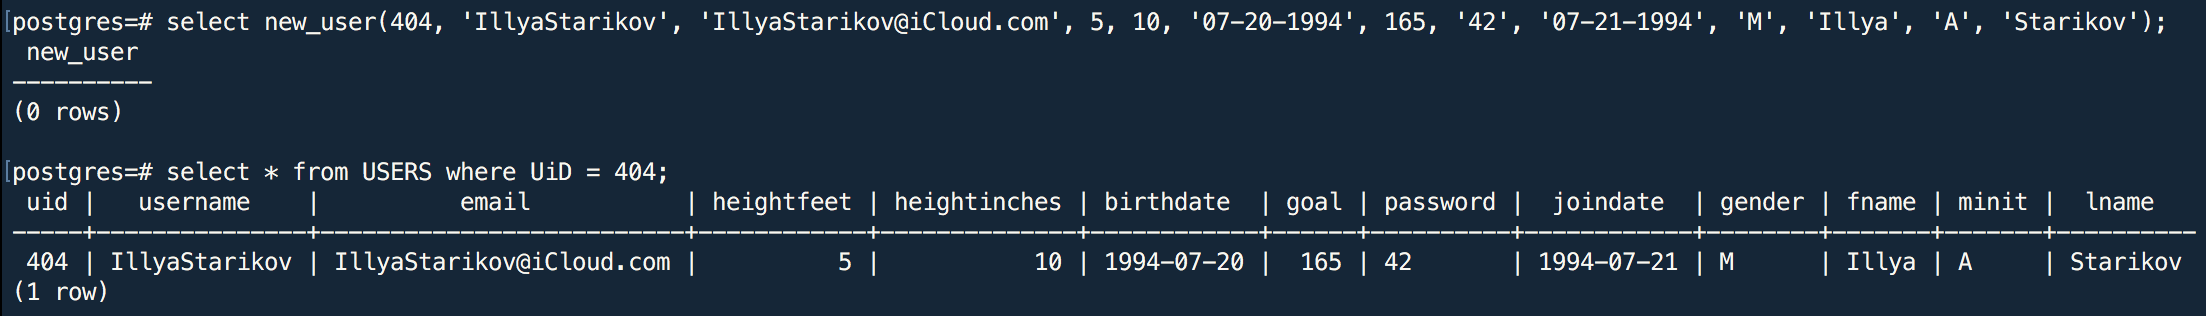
\includegraphics[width=\columnwidth]{include/assets/screenshots/new_user}
\end{center}